\subsection{Matched occlusion and calibration sensitivity}
\label{subsec:matched_geometry}

We compare pose-only fusion with geometry-assisted reconstruction on predictions from the same corrupted images, following the matched protocol of Section~\ref{subsec:controlled_protocol} and Supplementary Section~\ref{S-sec:c07_matched_geometry}: one SAM3D call supplies both the projected 2D keypoints and the 3D pose of the same person, all five frozen methods retain the same 64,440 windows, and scoring uses the common 13 joints after all-15 canonicalization. This seven-condition study uses fresh paired predictions and a different joint subset from the preceding 18-condition study, so their numbers are not interchangeable.

\begin{table}[htbp]
\centering
\caption{Matched RGB-occlusion comparison on Unity, with supplied calibration and no added extrinsic perturbation. Common-13 canonical MPJPE (lower is better), on all 64,440 windows. Ratios select joints for patch placement, not image-area coverage.}
\label{tab:c07_occlusion_mpjpe}
\small
\setlength{\tabcolsep}{4pt}
\begin{tabular}{lrrrrr}
\toprule
Condition & CanonFuse3D & Average & DLT & Gated DLT & DLT-residual \\
\midrule
Clean & 0.1553 & 0.2797 & 0.2004 & 0.2108 & 0.0988 \\
Left 0.5 & 0.2103 & 0.3051 & 0.2542 & 0.2606 & 0.1498 \\
Right 0.5 & 0.1949 & 0.2890 & 0.2488 & 0.2556 & 0.1417 \\
Both 0.5 & 0.2514 & 0.3146 & 0.2957 & 0.2983 & 0.1870 \\
Left 1.0 & 0.4654 & 0.3992 & 0.4499 & 0.4495 & 0.3569 \\
Right 1.0 & 0.3706 & 0.3347 & 0.5501 & 0.4569 & 0.4070 \\
Both 1.0 & 0.5986 & 0.4654 & 0.5121 & 0.4866 & 0.4155 \\
\bottomrule
\end{tabular}
\par\smallskip\begin{minipage}{\linewidth}\footnotesize CanonFuse3D and canonical averaging use only predicted 3D. The three DLT-based methods additionally use estimated 2D and calibration. DLT follows~\cite{hartley2004multiple}; gating and the residual MLP are study-specific controls, not reproductions of published learned triangulation systems.\end{minipage}
\end{table}



With unperturbed supplied calibration (Table~\ref{tab:c07_occlusion_mpjpe}), DLT-residual has the lowest MPJPE in six of seven conditions: its clean error is 0.0988 versus 0.1553 for CanonFuse3D, and under the three ratio-0.5 masks its MPJPE is 25.6--28.8\% lower, whereas CanonFuse3D has 1.8--9.5\% lower PA-MPJPE and 43.7--46.0\% lower acceleration error. The additional-input method thus improves position accuracy, while the pose-only method retains advantages on aligned configuration and temporal second-difference error. CanonFuse3D also improves MPJPE over canonical averaging by 20.1--32.5\% under ratio-0.5 masks, but at ratio 1.0 this advantage reverses by 10.7--28.6\% for single-side and bilateral masking alike; the results do not support automatic rejection of an arbitrarily degraded input view.

\begin{figure}[htbp]
\centering
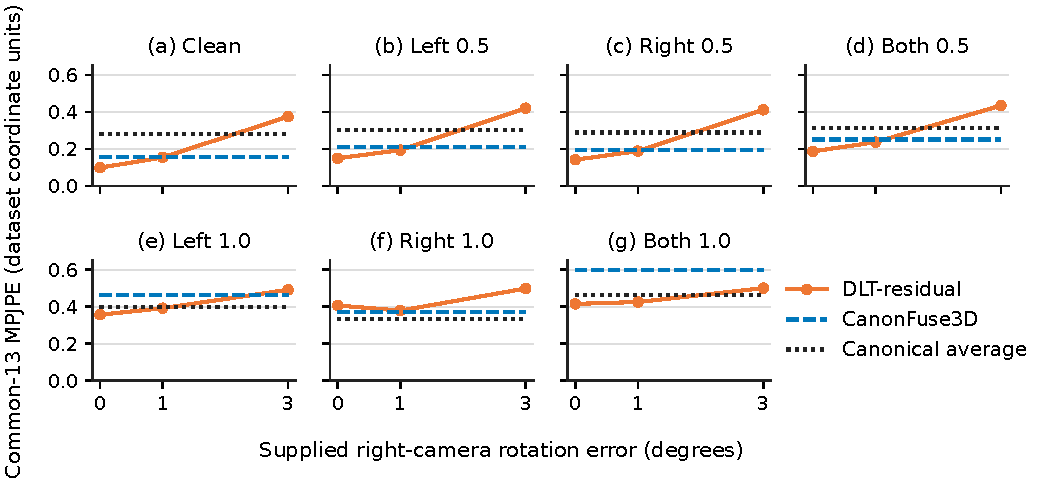
\includegraphics[width=\linewidth]{figures/extension/c07_calibration_sensitivity.pdf}
\caption{Calibration sensitivity across the seven matched conditions. Markers show DLT-residual~\cite{hartley2004multiple} at the three tested angles; pose-only references are unchanged. The synthetic rotation affects only the supplied right-camera orientation (values in Supplementary Table~\ref{S-tab:c07_calibration_mpjpe}).}
\label{fig:c07_calibration}
\end{figure}

Figure~\ref{fig:c07_calibration} shows the effect of perturbing the supplied right-camera extrinsics by $0^\circ$, $1^\circ$, and $3^\circ$ with the left camera and the right-camera center fixed. DLT-residual still has lower MPJPE than CanonFuse3D on clean and ratio-0.5 inputs at $1^\circ$. At $3^\circ$, CanonFuse3D has the lowest MPJPE and PA-MPJPE among the five methods on those four conditions, whereas canonical averaging is best on both metrics in all three ratio-1.0 conditions. Pose-only scores are invariant because neither their images nor their 3D inputs change; the experiment measures sensitivity to supplied calibration, not to physically moving a camera.

Missing observations remain in all denominators. At bilateral ratio 1.0, at least one view fails in 54.85\% of pair--frame positions, and after the batch-referenced transformation 33.30\% of CanonFuse3D and 70.05\% of DLT and gated-DLT frames have collapsed common-13 configurations, since a missing reference frame can affect an entire batch. These results characterize the coupled front-end, fallback, normalization, and prediction pipeline.

\FloatBarrier
